\begin{figure}[!h]
\begin{minipage}{0.45\textwidth}
    \centering
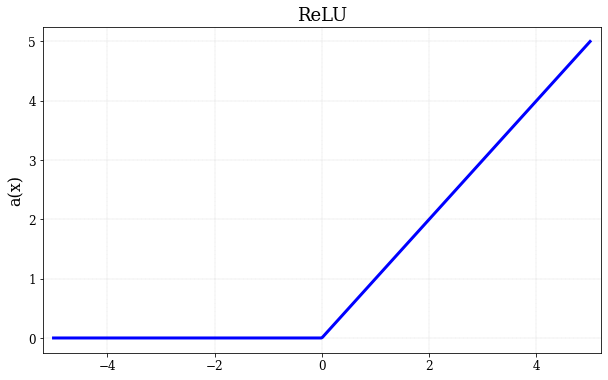
\includegraphics[width=\textwidth]{sections/03/Images/ReLU.png}
\caption{ReLU activation function}
    \label{fig:act_relu}
\end{minipage}
\hfill
\begin{minipage}{0.5\textwidth}
    \textbf{Rectified Linear Unit (ReLU)}
   \begin{align}
        a(x) &=
        \begin{cases}
        x   & \text{if } x > 0 \\
        0  & \text{if } x \leq 0 
  \end{cases}
\end{align}
The ReLU \cite{relu} is a continuous function with a point of non differentiability at 0. Despite being non differentiable - which is a point required for the back propagation step - this function is still implemented, mostly in the hidden layers of a network, due to its fast computation time. 
\end{minipage}
\end{figure}  


\begin{figure}[!h]

\begin{minipage}{0.5\textwidth}
    \textbf{Exponential Linear Unit (ELU)}
   \begin{align}
        a(x) &= 
        \begin{cases}
        \alpha \left(e^x -1\right)  & \text{if } x \leq 0 \\
        x  & \text{if } x > 0 
  \end{cases}
\end{align}
The ELU\cite{elu} activation functions is an improvement over the ReLU. In this case the negative values have an actual activation instead of being set to zero which may help the estimation of the network parameters. The drawback of choosing this function is an increase in the computational cost since an exponential operation is included. 
\end{minipage}
\hfill
\begin{minipage}{0.45\textwidth}
    \centering
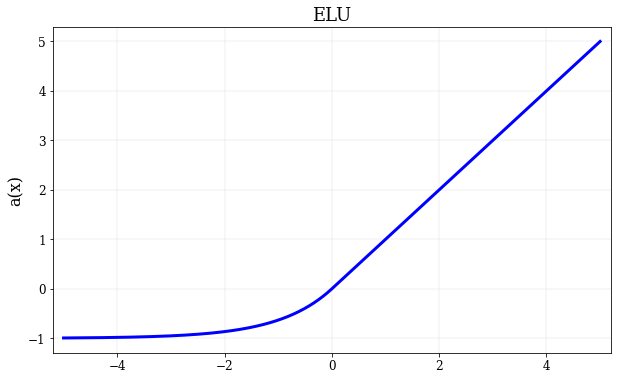
\includegraphics[width=\textwidth]{sections/03/Images/ELU.png}
\caption{ELU activation function}
    \label{fig:elu}
\end{minipage}
\end{figure}  


\begin{figure}[!h]
\begin{minipage}{0.45\textwidth}
    \centering
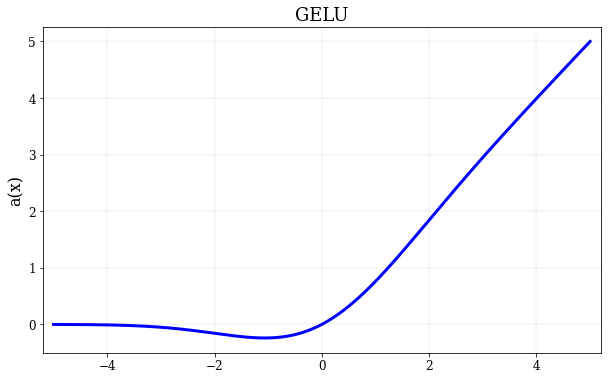
\includegraphics[width=\textwidth]{sections/03/Images/GELU.png}
\caption{GELU activation function}
    \label{fig:gelu}
\end{minipage}
\hfill
\begin{minipage}{0.5\textwidth}
    \textbf{Gaussian Error Linear Unit (GELU)}
   \begin{equation}
       a(x) = \frac{1}{2} x \left( 1+\text{erf} \left( \frac{x}{\sqrt{2}}\right)\right)
   \end{equation}
   The GELU\cite{gelu} is one of the newest activation functions. It was implemented in some of the most recent Deep Learining applications proving to be one of the best activations in the Natural Language Processing field\cite{bert,gpt}. 
\end{minipage}
\end{figure}  


\begin{figure}[!h]
\begin{minipage}{0.5\textwidth}
    \textbf{Binary step} or \textbf{Binary}
      \begin{align}
        a(x) &=
        \begin{cases}
        1   & \text{if } x \geq 0 \\
        -1  & \text{if } x < 0 
  \end{cases}
\end{align}
Neurons using this function are also called linear threshold units (LTU). This type of neurons can be used for solving simple tasks, but are not able to solve complex tasks like multiclass classifications. Often used in the so called Binarized Neural Networks (BNN).
\end{minipage}
\hfill
\begin{minipage}{0.45\textwidth}

    \centering
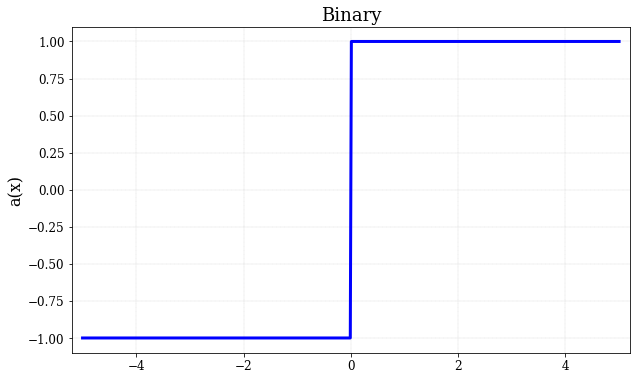
\includegraphics[width=\textwidth]{sections/03/Images/Binary.png}
\caption{Step activation function}
    \label{fig:act_step}
\end{minipage}
\end{figure}  


\begin{figure}[!h]
\begin{minipage}{0.45\textwidth}

    \centering
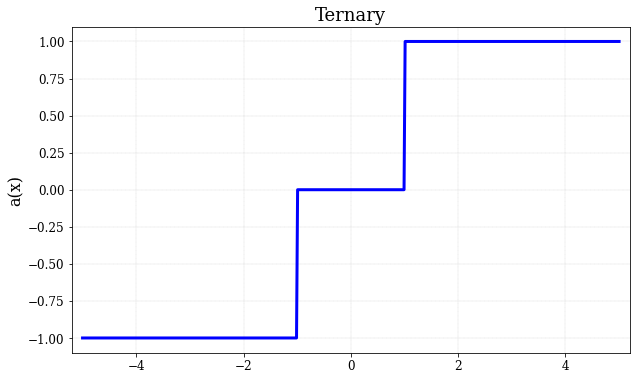
\includegraphics[width=\textwidth]{sections/03/Images/Ternary.png}
\caption{Ternary activation function}
    \label{fig:act_ter}
\end{minipage}
\hfill
\begin{minipage}{0.5\textwidth}
    \textbf{Ternary step} or \textbf{Ternary}
   \begin{align}
        a(x) &=
        \begin{cases}
        1   & \text{if } x \geq 1 \\
        0   & \text{if } -1 < x < 1 \\
        -1  & \text{if } x \leq -1
        \end{cases}
    \end{align}
   Quantized version of the hyperbolic tangent, employed mostly on the so-called Ternarized Neural Networks (TNN). Its usefulness lies on the fact that the operations can be mapped to trivial combinatorial ones. 
\end{minipage}
\end{figure}  


\begin{figure}[!h]

\begin{minipage}{0.5\textwidth}
    \textbf{Sigmoid} or \textbf{Soft step}
   \begin{equation}
       a(x) =\frac{1}{1+e^{-x}}
   \end{equation}
   The sigmoid function provides an output value in $[0,1]$ and it is differentiable in every point. This properties makes it one of the most used activation functions for the last layer of an ANN.
\end{minipage}
\hfill
\begin{minipage}{0.45\textwidth}

    \centering
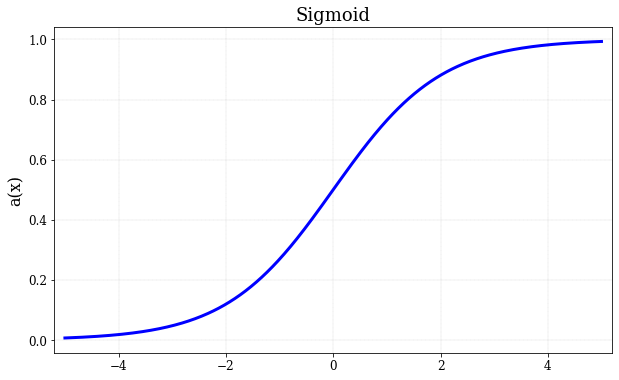
\includegraphics[width=\textwidth]{sections/03/Images/Sigmoid.png}
\caption{Sigmoid activation function}
    \label{fig:act_sig}
\end{minipage}
\end{figure}  


\begin{figure}[h!]
\begin{minipage}{0.45\textwidth}
    \centering
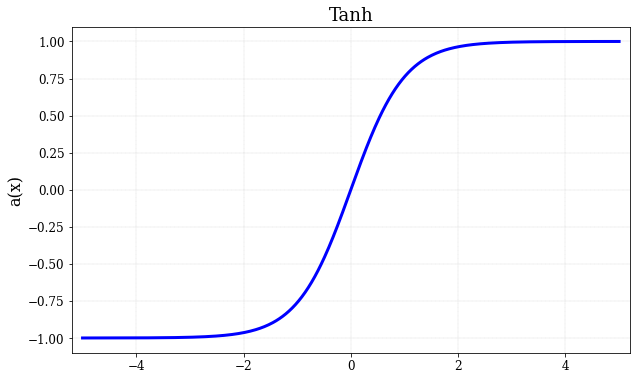
\includegraphics[width=\textwidth]{sections/03/Images/Tanh.png}
\caption{Hyperbolic tangent activation function}
    \label{fig:act_tanh}
\end{minipage}
\hfill
\begin{minipage}{0.5\textwidth}
    \textbf{Hyperbolic tangent}
   \begin{equation}
       a(x) =\frac{e^x-e^{-x}}{e^x+e^{-x}}
   \end{equation}
The hyperbolic tangent has similar properties to the sigmoid function. Its output is however in $[-1,1]$ which may speed up convergence in some applications.
\end{minipage}
\end{figure} 

\begin{figure}[h!]
\textbf{Softmax} \\

\begin{equation}
       a_i(\bold{x}) =\frac{e^{x_i}}{\sum_{j=1}^{K} e^{x_j}}
   \end{equation}
 
The softmax function takes as input a vector $\bold{x}$ of $K$ real numbers, and normalizes it into a probability distribution consisting of K probabilities proportional to the exponentials of the input numbers. After applying softmax, each component will be in the interval $\left(0,1\right)$ and the components will add up to 1, so that they can be interpreted as probabilities. Furthermore, the larger input components will correspond to larger probabilities. Generally used for multi-class classification.

\end{figure}

\vfill

